\documentclass[a4paper,14pt]{article} % формат документа

\usepackage{cmap} % поиск в ПДФ
\usepackage[T2A]{fontenc} % кодировка
\usepackage[utf8]{inputenc} % кодировка исходного текста
\usepackage[english,russian]{babel} % локализация и переносы
\usepackage[left = 2cm, right = 1cm, top = 2cm, bottom = 2 cm]{geometry} % поля
\usepackage{listings}
\usepackage{graphicx} % для вставки рисунков
\usepackage{amsmath}
\graphicspath{{pictures/}}
\DeclareGraphicsExtensions{.pdf,.png,.jpg}
\newcommand{\anonsection}[1]{\section*{#1}\addcontentsline{toc}{section}{#1}}

\lstset{ %
	language=Python,                % Язык программирования 
	numbers=left,                   % С какой стороны нумеровать          
	frame=single,                    % Добавить рамку
}

\begin{document}
	\begin{titlepage}

       		\begin{center}
         		\large
		
        			Государственное образовательное учреждение высшего профессионального образования\\
       			“Московский государственный технический университет имени Н.Э.Баумана”
         		\vspace{3cm}
            
            		\textsc{Дисциплина: Анализ алгоритмов}
           		\vspace{0.5cm}
                
            		\textsc{Лабораторная работа № 5}
           		 \vspace{3cm}
            
           		 \LARGE 
		 
		 	Конвейерные вычисления
           		 \vspace{3cm}
            
            		\begin{flushright}
            			Студент: \\
				Сиденко Анастасия Генадьевна \\   
            			Группа: ИУ7-53Б \\
           			\hfill
            
           			Преподаватели: \\
				Строганов Юрий Владимирович \\
           			Волкова Лилия Леонидовна
            			\vfill
            		\end{flushright}
		
			\large
            		2019 г.
		\end{center}

	\end{titlepage}
    
	\tableofcontents
	
	\newpage
    
	\anonsection{Введение}
	\hfill
	
	Имеется большое количество важнейших задач, решение которых требует использования огромных вычислительных мощностей, зачастую недоступных для современных вычислительных систем. 
	
	 Постоянно появляются новые задачи подобного рода и возрастают требования к точности и к скорости решения прежних задач; поэтому вопросы разработки и использования сверхмощных компьютеров (называемых суперкомпьютерами) актуальны сейчас и в будущем.[1] Но пока эти трудности пока что не удается преодолеть. Из-за этого приходится и эти по пути создания параллельных вычислительных систем, т.е. систем, в которых предусмотрена одновременная реализация ряда вычислительных процессов, связанных с решением одной задачи.[2] На современном этапе развития вычислительной техники такой способ, по-видимому, является одним из основных способов ускорения вычислений.
	 
	 Многие явления природы характеризуются параллелизмом (одновременным исполнением процессов с применением различных путей и способов). В частности, в живой природе параллелизм распространен очень широко в дублирующих системах для получения надежного результата. Параллельные процессы пронизывают общественные отношения, ими характеризуются развитие науки, культуры и экономики в человеческом обществе. Среди этих процессов особую роль играют параллельные информационные потоки. [3]
	 
	 Среди параллельных систем различают конвейерные, векторные, матричные, систолические, спецпроцессоры и т.п. В данной работе используются конвейерные. [2]
	 
	 В данной работе стоит задача реализации алгоритма деления чисел с плавающей запятой, сравнение последовательной и конвейерное реализаций. 
		
	\newpage


        \section{Аналитическая часть}
        \hfill
        
        Одной из важнейших идей при создании многопроцессорных систем и при эффективной реализации алгоритмов на этих системах является идея конвейерных вычислений.
                
        
        \subsection{Описание задачи}
        \hfill
        
        Конвейеризация – это техника, в результате которой  задача или  команда разбивается  на некоторое число подзадач, которые  выполняются последовательно. Каждая  подкоманда   выполняется на своем логическом  устройстве.    Все     логические    устройства   (ступени)  соединяются последовательно таким образом, что выход  i-ой   ступени   связан   с   входом   (i+1)-ой   ступени,  все ступени  работают  одновременно.  Множество  ступеней называется    конвейером.    Выигрыш     во    времени достигается при  выполнении  нескольких задач  за  счет параллельной   работы   ступеней,  вовлекая  на  каждом такте новую задачу или команду.[4]

	В конвейере различают r последовательных этапов, так что когда $i$-я операция проходит $s$-й этап, то $(i+k)$-я операция проходит $(s-k)$-й этап (рис. 1).
	
	\begin{center}
		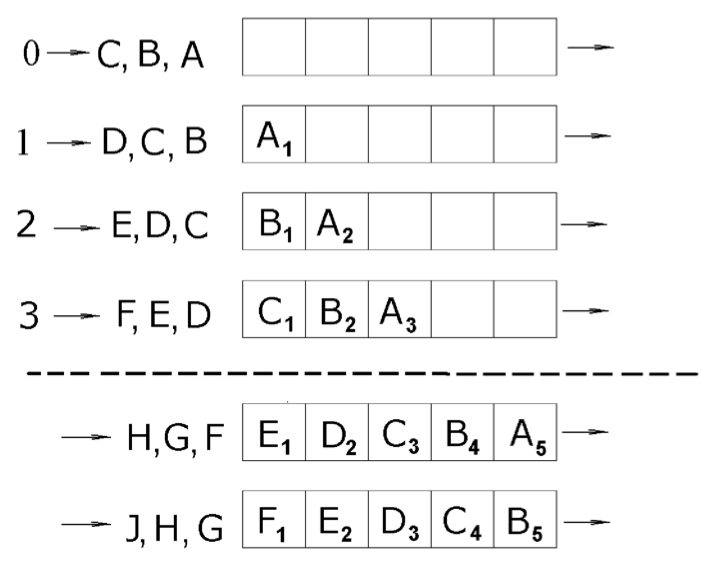
\includegraphics[scale = 0.8]{img1} \\ Рис.  1 - Схема конвейера. 
	\end{center}
	
	В данной работе реализован алгоритм деления чисел с плавающей запятой, состоящих из знака, порядка и мантиссы. 
        	                
        \subsection{Выводы} 
        \hfill
        
        Таким образом, выигрыш     во    времени достигается при  выполнении  нескольких задач  за  счет параллельной   работы   ступеней,  вовлекая  на  каждом такте новую задачу или команду. Однако работу конвейера тормозят зависимости  по данным, конфликты по ресурсам. 

	\newpage

	\section{Конструкторская часть}
	\hfill
	
	Стоит задача конвейерных вычислений алгоритма деления чисел с плавающей запятой. 
		
	\subsection{Функциональная модель}
	
	На рисунке 2 представлена функциональная модель нашей задачи.  
	
	\begin{center}
		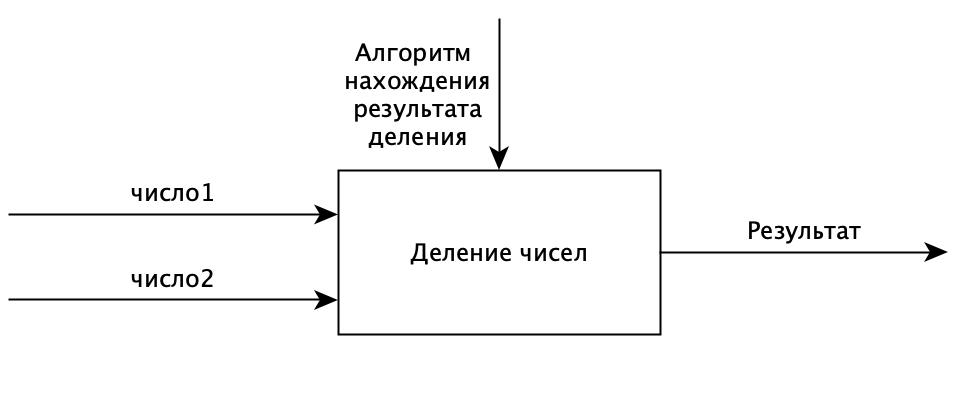
\includegraphics[scale = 0.8]{idef0} \\ Рис.  2 - Функциональная модель алгоритма нахождения произведения матриц. 
	\end{center}
	        
        \subsection{Схемы алгоритмов}
        \hfill
        
         Приведем схему алгоритма (см. рисунок 3), где каждое действие выполняется в отдельном потоке. 
         
        \hfill

	\hfill
	
	\begin{center}
        		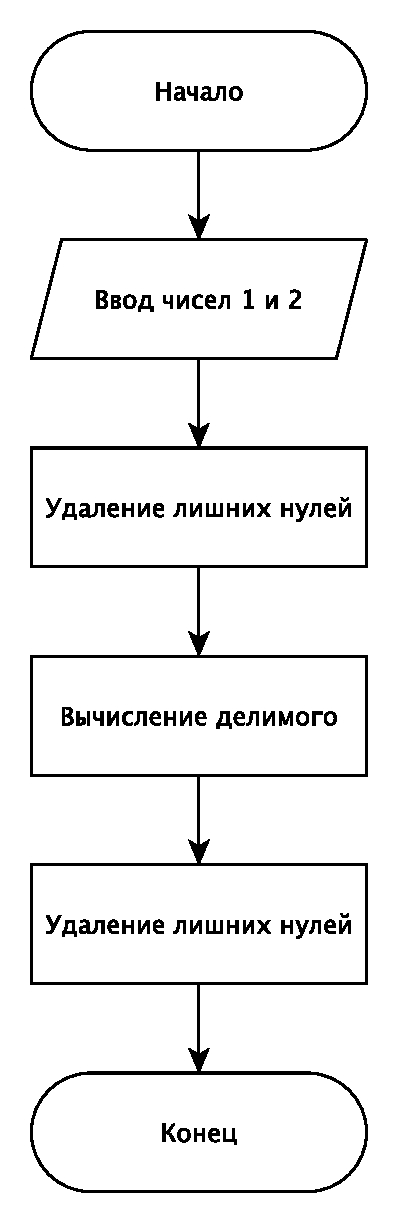
\includegraphics[scale = 0.53]{shema1} \\ Рис. 3 - Алгоритм работы с программы
	\end{center}
        	
	\subsection{Выводы}
	\hfill
	
	Описанный принцип построения процессора действительно напоминает конвейер сборочного завода, на котором изделие последовательно проходит ряд рабочих мест. На каждом из этих мест над изделием производится новая операция. Эффект ускорения достигается за счет одновременной обработки ряда изделий на разных рабочих местах.[6]
	
		
    	\newpage

        \section{Технологическая часть}
        \hfill
        
        Необходимо изучить и реализовать конвейерную обработку процесса деления чисел. 
        
        \subsection{Требования к программному обеспечению}
        \hfill
        
        ПО должно предоставлять возможность замеров процессорного времени выполнения реализации каждого алгоритма. Требуется провести замеры для варьирующегося количества чисел. Один эксперимент ставится не менее 5 раз, результат одного эксперимента рассчитывается как среднее значение результатов проведенных испытаний с одинаковыми входными данными.
        \hfill
        
        \subsection{Средства реализации}
        \hfill
        
        В качестве языка программирования был выбран С++, так как я знакома с этих языком программирования и он удовлетворяет требованиям об необходимости использовании нативных потоков. [11]
        \hfill
        
        Для замеров времени была выбран метод $high\_resolution\_clock::now()$, возвращает текущее время процессора как число тиков, выраженное в микросекундах в Unix.[5]
        \hfill
        
        Для генерации случайных чисел использовался метод $rand()$. 
        
        Для работы с потоками использована библиотека $<thread>$. 
        \hfill
        
        \subsection{Листинг кода}
        \hfill
        
        Код алгоритма деления чисел с плавающей запятой с помощью конвейерных вычислений представлен на листингах 1-6. 
        
\begin{lstlisting}[caption=Чтение 1 числа]
void thread1() {
  Builder builder;

  while (true) {
    if (str1.empty()) {
      sign++;
      return;
    }
    builder.build_number(str1.front());
    str1.pop();
    cout_lock.lock();
    cout << 1 << ' ' << builder.get_result() << endl;
    cout_lock.unlock();
    if (!builder.get_result().error) {
      data_lock.lock();
      nulesnumber1.push(builder.get_result());
      data_lock.unlock();
    }
  }
}
\end{lstlisting}

\begin{lstlisting}[caption=Чтение 2 числа]
void thread2() {
  Builder builder;

  while (true) {
    if (str2.empty()) {
      sign++;
      return;
    }
    builder.build_number(str2.front());
    str2.pop();
    cout_lock.lock();
    cout << 2 << ' ' << builder.get_result() << endl;
    cout_lock.unlock();
    if (!builder.get_result().error) {
      data_lock.lock();
      nulesnumber2.push(builder.get_result());
      data_lock.unlock();
    }
  }
}
\end{lstlisting}

\begin{lstlisting}[caption=Удаление незначаших нулей из числа 1]
void thread3() {
  Long_number num;

  while (true) {
    if (nulesnumber1.empty()) {
      if (sign >= 2) {
        sign++;
        return;
      }
      continue;
    }
    num = nulesnumber1.front();
    data_lock.lock();
    nulesnumber1.pop();
    data_lock.unlock();
    num.insignificant_nules();

    cout_lock.lock();
    cout << 3 << ' ' << num << endl;
    cout_lock.unlock();
    data_lock.lock();
    number1.push(num);
    data_lock.unlock();
  }
}
\end{lstlisting}

\begin{lstlisting}[caption=Удаление незначаших нулей из числа 2]
void thread4() {
  Long_number num;

  while (true) {
    if (nulesnumber2.empty()) {
      if (sign >= 3) {
        sign++;
        return;
      }
      continue;
    }
    num = nulesnumber2.front();
    data_lock.lock();
    nulesnumber2.pop();
    data_lock.unlock();
    num.insignificant_nules();

    cout_lock.lock();
    cout << 4 << ' ' << num << endl;
    cout_lock.unlock();
    data_lock.lock();
    number2.push(num);
    data_lock.unlock();
  }
}
\end{lstlisting}

\begin{lstlisting}[caption=Деление]
void thread5() {
  Long_number num;

  while (true) {
    if (number1.empty() || number2.empty()) {
      if (sign >= 4) {
        sign++;
        return;
      }
      continue;
    }
    num.division(number1.front(), number2.front());
    data_lock.lock();
    number1.pop();
    number2.pop();
    data_lock.unlock();

    cout_lock.lock();
    cout << 5 << ' ' << num << endl;
    cout_lock.unlock();
    if (!num.error) {
      data_lock.lock();
      nulesnumber.push(num);
      data_lock.unlock();
    }
  }
}
\end{lstlisting}

\begin{lstlisting}[caption=Удаление незначаших нулей из результата]
void thread6() {
  Long_number num;
  while (true) {
    if (nulesnumber.empty()) {
      if (sign >= 5) {
        sign++;
        return;
      }
      continue;
    }
    num = nulesnumber.front();
    data_lock.lock();
    nulesnumber.pop();
    data_lock.unlock();
    num.insignificant_nules();

    cout_lock.lock();
    cout << 6 << ' ' << num;
    cout_lock.unlock();
  }
}
\end{lstlisting}
        
	
 	\subsection{Выводы}
	\hfill
	
	Описанный принцип построения процессора действительно напоминает конвейер. На каждой из лент производится новая операция. Эффект ускорения достигается за счет одновременной обработки нескольких операций на разных лентах конвейера.
        
        \newpage
        

        \section{Экспериментальная часть}
        \hfill
        
       Стоит задача разработки и сравнительного анализа алгоритмов, вычисляющих деление чисел с плавающей запятой последовательным и конвейерным способом.
       
       В реализациях в целях увеличения точности подсчета времени вывод был вынесен за пределы функций-алгоритмов. В целях наглядности были опущены части программ, не относящиеся к работе алгоритмов.


        \subsection{Примеры работы}
	\hfill
	
	На рисунке 4 представлены примеры работы программы на разных входных данных. В параметрах командной строки можно указать желаемое число количества чисел, по умолчанию 1.
	\begin{figure}[ht]\center
		\begin{tabular}{cc}
			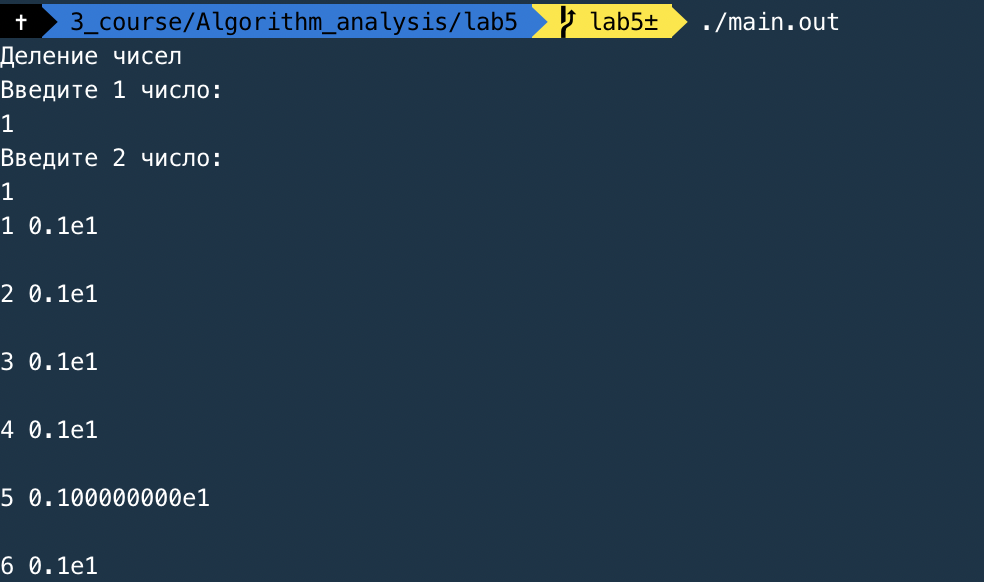
\includegraphics[width=80mm]{ex1} & 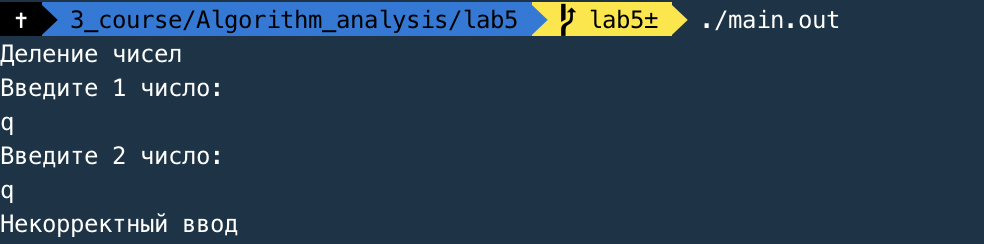
\includegraphics[width=80mm]{ex2} \\
			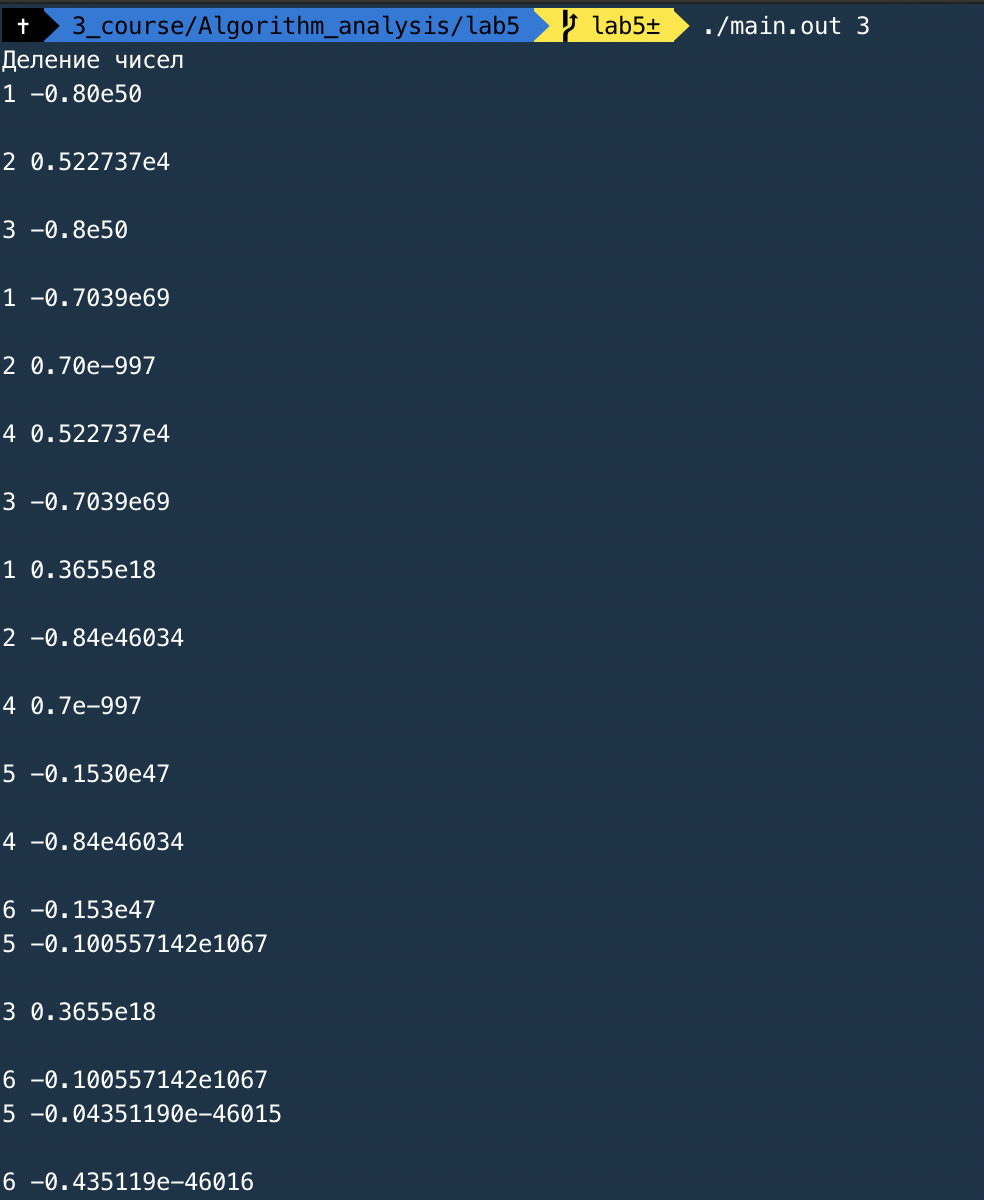
\includegraphics[width=80mm]{ex3} & 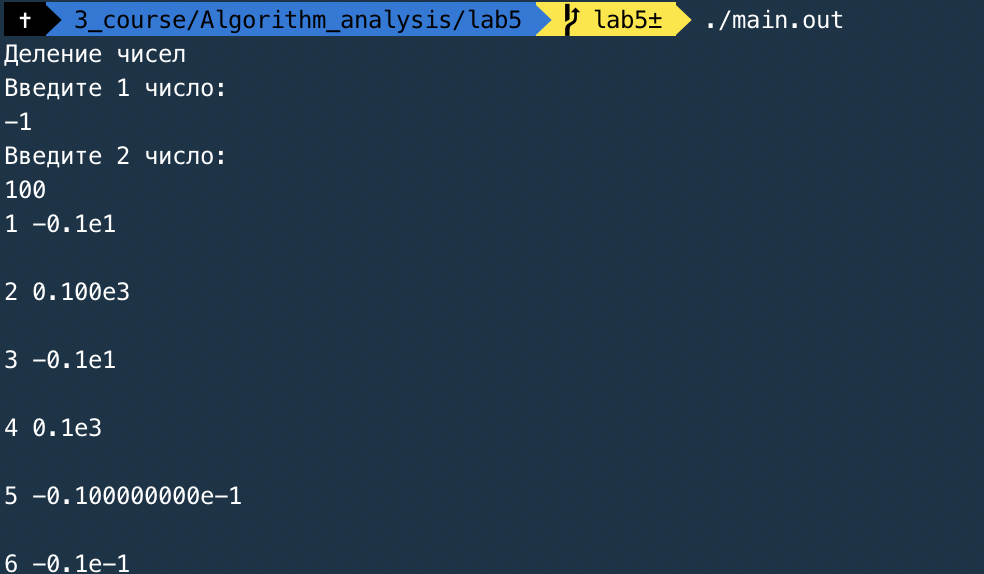
\includegraphics[width=80mm]{ex4}
		\end{tabular}
		\\ Рис. 4 - Примеры работы
	\end{figure}
	

	\subsection{Замеры времени}
	\hfill
	
	На графике 5 представлено сравнение алгоритмов умножения матриц. 
	\begin{center}
        		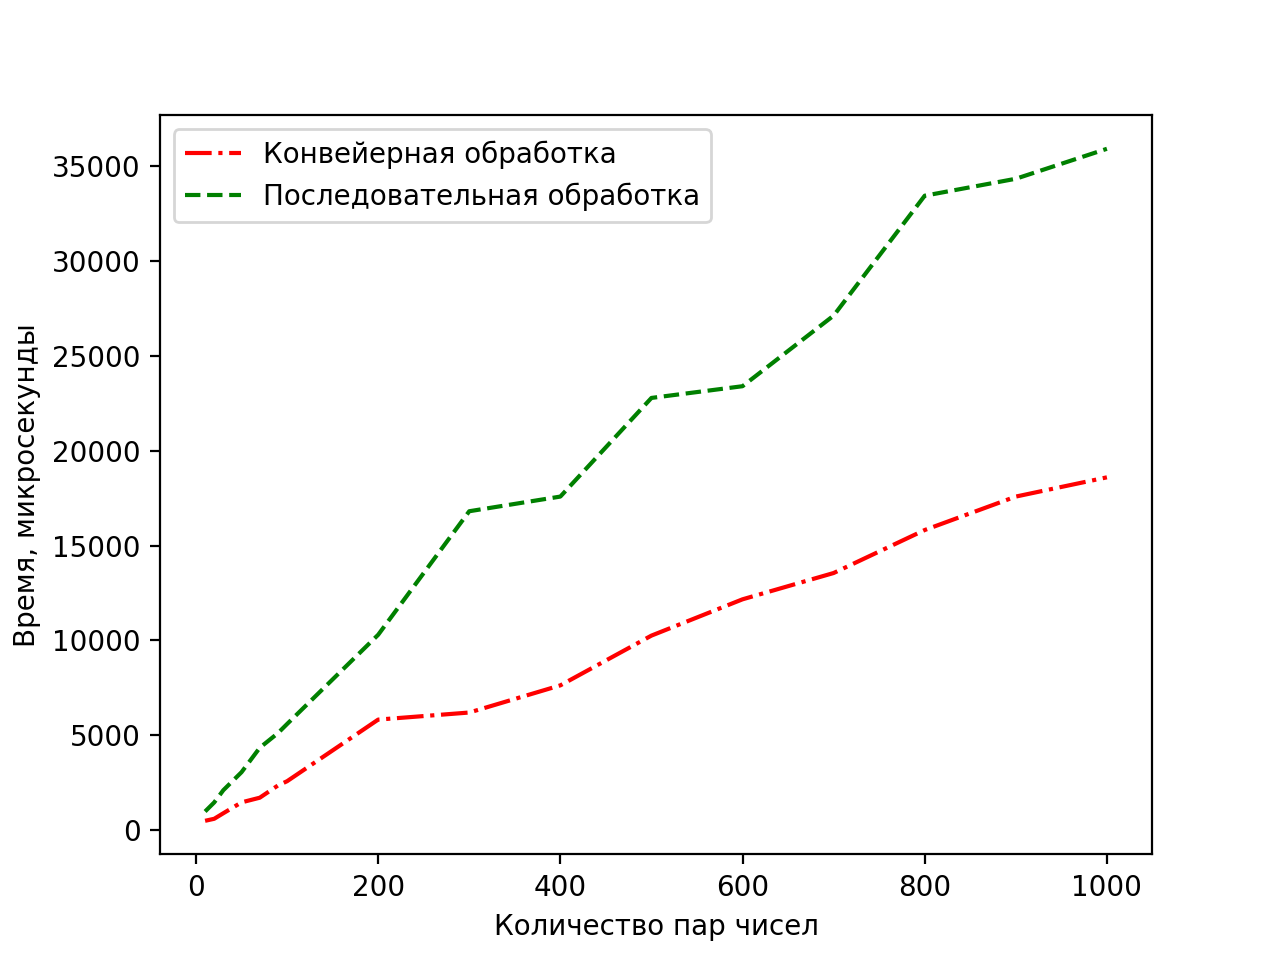
\includegraphics[scale = 1]{graph} \\ Рис. 5 - Сравнение реализации алгоритмов нахождения делимого чисел с плавающей запятой
	\end{center}

	\subsection{Выводы}
	\hfill
	
	 Таким образом, выигрыш    во    времени достигается при  выполнении  нескольких задач  за  счет параллельной   работы   ступеней,  вовлекая  на  каждом такте новую задачу или команду. Однако работу конвейера тормозят зависимости  по данным, конфликты по ресурсам. 
	
	\newpage

        \anonsection{Заключение}
        \hfill
        
        В данной работе реализован алгоритм деления чисел с плавающей запятой и проведено сравнение последовательной и конвейерной реализаций. 
        
        Ступени такого конвейера выполняются последовательно, а операции одной ступени параллельно. Теория, на основе параллельно-последовательной схемы, позволяет аналитически вычислять основные характеристики конвейерного процесса и составлять расписание процесса. Модели конвейерных процессов, в той или иной модификации, широко используются для решения различных прикладных задач. 
        
        Однако при небольших вычисления, из-за блокировки ресурсов и передачи данных между потоками, конвейерная обработка проигрывает последовательной. 
       
 	\newpage

        \begin{thebibliography}{}
        		\bibitem{} Воеводин В.В. Математические модели и методы в парал- лельных процессах. М., 1986. 296 с.
		\bibitem{}  Корнеев В.В. Параллельные вычислительные системы. М., 1999. 320 с.
		
		\bibitem{}  Yukiya Aoyama, Jun Nakano. RS/6000 SP:Practical MPI Programming. IBM. Technical Support Organization., 2000. 221
		
		\bibitem{}  [Электронный ресурс]. - Режим доступа: http://www.myshared.ru/slide/674082/(дата обращения: 05.11.2019)
		
		\bibitem{}  [Электронный ресурс]. - Режим доступа: https://en.cppreference.com/w/cpp/chrono/duration/durationcast(дата обращения: 22.10.2019)
		
		\bibitem{} [Электронный ресурс] - Режим доступа: https://studref.com/313869/informatika/konveyerizatsiyavychisleniy (дата обращения: 05.11.2019)
	
		\bibitem{} [Электронный ресурс] - Режим доступа: https://cyberleninka.ru/article/n/primenenie-modeli-konveyernyh-protsessov-rekursivnogo-tipa-dlya-resheniya-prikladnyh-zadach (дата обращения: 05.11.2019)
	\end{thebibliography} 

\end{document}
